% CVPR 2025 Paper Template; see https://github.com/cvpr-org/author-kit

\documentclass[10pt,twocolumn,letterpaper]{article}
\usepackage{graphicx}
\usepackage{float}
%%%%%%%%% PAPER TYPE  - PLEASE UPDATE FOR FINAL VERSION
% \usepackage{cvpr}              % To produce the CAMERA-READY version
\usepackage[review]{cvpr}      % To produce the REVIEW version
% \usepackage[pagenumbers]{cvpr} % To force page numbers, e.g. for an arXiv version

% Import additional packages in the preamble file, before hyperref
%
% --- inline annotations
%
\newcommand{\red}[1]{{\color{red}#1}}
\newcommand{\todo}[1]{{\color{red}#1}}
\newcommand{\TODO}[1]{\textbf{\color{red}[TODO: #1]}}
% --- disable by uncommenting  
% \renewcommand{\TODO}[1]{}
% \renewcommand{\todo}[1]{#1}



% It is strongly recommended to use hyperref, especially for the review version.
% hyperref with option pagebackref eases the reviewers' job.
% Please disable hyperref *only* if you encounter grave issues, 
% e.g. with the file validation for the camera-ready version.
%
% If you comment hyperref and then uncomment it, you should delete *.aux before re-running LaTeX.
% (Or just hit 'q' on the first LaTeX run, let it finish, and you should be clear).
\definecolor{cvprblue}{rgb}{0.21,0.49,0.74}
\usepackage[pagebackref,breaklinks,colorlinks,allcolors=cvprblue]{hyperref}

%%%%%%%%% PAPER ID  - PLEASE UPDATE
\def\paperID{*****} % *** Enter the Paper ID here
\def\confName{CVPR}
\def\confYear{2025}

%%%%%%%%% TITLE - PLEASE UPDATE
%\title{\LaTeX\ Author Guidelines for \confName~Proceedings}
%中期报告:时间序列预测——长周期预测
\title{Interim Report: Time Series Forecasting - Long period forecasting}
%%%%%%%%% AUTHORS - PLEASE UPDATE
\author{First Author\\
Institution1\\
Institution1 address\\
{\tt\small firstauthor@i1.org}
% For a paper whose authors are all at the same institution,
% omit the following lines up until the closing ``}''.
% Additional authors and addresses can be added with ``\and'',
% just like the second author.
% To save space, use either the email address or home page, not both
\and
Second Author\\
Institution2\\
First line of institution2 address\\
{\tt\small secondauthor@i2.org}
}

\begin{document}
\maketitle
\begin{abstract}
%	对于寿命较长的电子原件,如10年、20年等,我们不可能实实在在地检测其寿命,直到其损坏。经济的做法是对其寿命进行预测。在本文中,我们利用收集的一类电子管的、其电流的时间序列数据,预测其寿命情况。我们使用LSTM、TCN、GRU、RNN、MLP作为Batchmark,探究Autoformer以及Timesnet在此类问题上的性能,并尝试做出改进
For electronic components with a long life, such as 10 years, 20 years, etc., it is impossible for us to actually detect its data until it is damaged. The economic way to do this is to make predictions about its lifespan. In this paper, we use the time series data collected from a kind of electron tube and its current to predict its lifetime. We use LSTM, TCN, GRU, RNN, MLP as batchmark to explore the performance of Autoformer as well as Timesnet on such problems and try to make improvements
\end{abstract}    
\section{Introduction}
\label{sec:intro}
% 时间序列预测已被广泛应用于经济规划、交通路况预测、天气预报、能源消耗以及疾病传播预测等方方面面。其中,一个醒目的需求是,将预测的时间延长到更长远的未来,这有利于超长期的规划和预警。因此,在本文中,我们研究了时间序列的长期预测问题。一些电子原件的寿命可长达数十年,然而一旦损坏,却可能是任何一个未知的时间。为了某一个具体的电子元件的寿命,我们必须对其现有的工作情况的数据进行分析,从而得到其在未来工作中最可能的寿命。在本文中,我们挑选了一类微波电子管作为研究对象。其在工作中有一个期望的电流值,随着时间的推移,在工作条件下,电流值将越来越低,直至低于期望电流值的90%,此时该电子管则被视为报废。

Time series forecasting has been widely used in economic planning, traffic condition forecasting, weather forecasting, energy consumption and disease transmission forecasting. Among them, a striking need is to extend the forecast time into the longer future, which facilitates ultra-long-term planning and early warning. Therefore, in this paper, we study the problem of long-term forecasting for time series. The life of some electronic components can be as long as decades, but once damaged, it may be any unknown time. For the life of a specific electronic component, we must analyze the data of its existing working condition, so as to obtain its most likely life in future work. In this paper, we select a class of microwave tubes as the research object. It has a desired current value in the work, with the passage of time, under the working conditions, the current value will be lower and lower, until less than 90\% of the desired current value, at this time the tube is regarded as scrapped.
%-------------------------------------------------------------------------
\subsection{Language}

All manuscripts must be in English.

\subsection{Dual submission}

Please refer to the author guidelines on the \confName\ \confYear\ web page for a
discussion of the policy on dual submissions.

\subsection{Paper length}
Papers, excluding the references section, must be no longer than eight pages in length.
The references section will not be included in the page count, and there is no limit on the length of the references section.
For example, a paper of eight pages with two pages of references would have a total length of 10 pages.
{\bf There will be no extra page charges for \confName\ \confYear.}

Overlength papers will simply not be reviewed.
This includes papers where the margins and formatting are deemed to have been significantly altered from those laid down by this style guide.
Note that this \LaTeX\ guide already sets figure captions and references in a smaller font.
The reason such papers will not be reviewed is that there is no provision for supervised revisions of manuscripts.
The reviewing process cannot determine the suitability of the paper for presentation in eight pages if it is reviewed in eleven.

%-------------------------------------------------------------------------
\subsection{The ruler}
The \LaTeX\ style defines a printed ruler which should be present in the version submitted for review.
The ruler is provided in order that reviewers may comment on particular lines in the paper without circumlocution.
If you are preparing a document using a non-\LaTeX\ document preparation system, please arrange for an equivalent ruler to appear on the final output pages.
The presence or absence of the ruler should not change the appearance of any other content on the page.
The camera-ready copy should not contain a ruler.
(\LaTeX\ users may use options of \texttt{cvpr.sty} to switch between different versions.)

Reviewers:
note that the ruler measurements do not align well with lines in the paper --- this turns out to be very difficult to do well when the paper contains many figures and equations, and, when done, looks ugly.
Just use fractional references (\eg, this line is $087.5$), although in most cases one would expect that the approximate location will be adequate.


\subsection{Paper ID}
Make sure that the Paper ID from the submission system is visible in the version submitted for review (replacing the ``*****'' you see in this document).
If you are using the \LaTeX\ template, \textbf{make sure to update paper ID in the appropriate place in the tex file}.


\subsection{Mathematics}

Please number all of your sections and displayed equations as in these examples:
\begin{equation}
  E = m\cdot c^2
  \label{eq:important}
\end{equation}
and
\begin{equation}
  v = a\cdot t.
  \label{eq:also-important}
\end{equation}
It is important for readers to be able to refer to any particular equation.
Just because you did not refer to it in the text does not mean some future reader might not need to refer to it.
It is cumbersome to have to use circumlocutions like ``the equation second from the top of page 3 column 1''.
(Note that the ruler will not be present in the final copy, so is not an alternative to equation numbers).
All authors will benefit from reading Mermin's description of how to write mathematics:
\url{http://www.pamitc.org/documents/mermin.pdf}.

\subsection{Blind review}

Many authors misunderstand the concept of anonymizing for blind review.
Blind review does not mean that one must remove citations to one's own work---in fact it is often impossible to review a paper unless the previous citations are known and available.

Blind review means that you do not use the words ``my'' or ``our'' when citing previous work.
That is all.
(But see below for tech reports.)

Saying ``this builds on the work of Lucy Smith [1]'' does not say that you are Lucy Smith;
it says that you are building on her work.
If you are Smith and Jones, do not say ``as we show in [7]'', say ``as Smith and Jones show in [7]'' and at the end of the paper, include reference 7 as you would any other cited work.

An example of a bad paper just asking to be rejected:
\begin{quote}
\begin{center}
    An analysis of the frobnicatable foo filter.
\end{center}

   In this paper we present a performance analysis of our previous paper [1], and show it to be inferior to all previously known methods.
   Why the previous paper was accepted without this analysis is beyond me.

   [1] Removed for blind review
\end{quote}


An example of an acceptable paper:
\begin{quote}
\begin{center}
     An analysis of the frobnicatable foo filter.
\end{center}

   In this paper we present a performance analysis of the  paper of Smith \etal [1], and show it to be inferior to all previously known methods.
   Why the previous paper was accepted without this analysis is beyond me.

   [1] Smith, L and Jones, C. ``The frobnicatable foo filter, a fundamental contribution to human knowledge''. Nature 381(12), 1-213.
\end{quote}

If you are making a submission to another conference at the same time, which covers similar or overlapping material, you may need to refer to that submission in order to explain the differences, just as you would if you had previously published related work.
In such cases, include the anonymized parallel submission~\cite{Authors14} as supplemental material and cite it as
\begin{quote}
[1] Authors. ``The frobnicatable foo filter'', F\&G 2014 Submission ID 324, Supplied as supplemental material {\tt fg324.pdf}.
\end{quote}

Finally, you may feel you need to tell the reader that more details can be found elsewhere, and refer them to a technical report.
For conference submissions, the paper must stand on its own, and not {\em require} the reviewer to go to a tech report for further details.
Thus, you may say in the body of the paper ``further details may be found in~\cite{Authors14b}''.
Then submit the tech report as supplemental material.
Again, you may not assume the reviewers will read this material.

Sometimes your paper is about a problem which you tested using a tool that is widely known to be restricted to a single institution.
For example, let's say it's 1969, you have solved a key problem on the Apollo lander, and you believe that the 1970 audience would like to hear about your
solution.
The work is a development of your celebrated 1968 paper entitled ``Zero-g frobnication: How being the only people in the world with access to the Apollo lander source code makes us a wow at parties'', by Zeus \etal.

You can handle this paper like any other.
Do not write ``We show how to improve our previous work [Anonymous, 1968].
This time we tested the algorithm on a lunar lander [name of lander removed for blind review]''.
That would be silly, and would immediately identify the authors.
Instead write the following:
\begin{quotation}
\noindent
   We describe a system for zero-g frobnication.
   This system is new because it handles the following cases:
   A, B.  Previous systems [Zeus et al. 1968] did not  handle case B properly.
   Ours handles it by including a foo term in the bar integral.

   ...

   The proposed system was integrated with the Apollo lunar lander, and went all the way to the moon, don't you know.
   It displayed the following behaviours, which show how well we solved cases A and B: ...
\end{quotation}
As you can see, the above text follows standard scientific convention, reads better than the first version, and does not explicitly name you as the authors.
A reviewer might think it likely that the new paper was written by Zeus \etal, but cannot make any decision based on that guess.
He or she would have to be sure that no other authors could have been contracted to solve problem B.
\medskip

\noindent
FAQ\medskip\\
{\bf Q:} Are acknowledgements OK?\\
{\bf A:} No.  Leave them for the final copy.\medskip\\
{\bf Q:} How do I cite my results reported in open challenges?
{\bf A:} To conform with the double-blind review policy, you can report results of other challenge participants together with your results in your paper.
For your results, however, you should not identify yourself and should not mention your participation in the challenge.
Instead present your results referring to the method proposed in your paper and draw conclusions based on the experimental comparison to other results.\medskip\\

\begin{figure}[t]
  \centering
  \fbox{\rule{0pt}{2in} \rule{0.9\linewidth}{0pt}}
   %\includegraphics[width=0.8\linewidth]{egfigure.eps}

   \caption{Example of caption.
   It is set in Roman so that mathematics (always set in Roman: $B \sin A = A \sin B$) may be included without an ugly clash.}
   \label{fig:onecol}
\end{figure}

\subsection{Miscellaneous}

\noindent
Compare the following:\\
\begin{tabular}{ll}
 \verb'$conf_a$' &  $conf_a$ \\
 \verb'$\mathit{conf}_a$' & $\mathit{conf}_a$
\end{tabular}\\
See The \TeX book, p165.

The space after \eg, meaning ``for example'', should not be a sentence-ending space.
So \eg is correct, {\em e.g.} is not.
The provided \verb'\eg' macro takes care of this.

When citing a multi-author paper, you may save space by using ``et alia'', shortened to ``\etal'' (not ``{\em et.\ al.}'' as ``{\em et}'' is a complete word).
If you use the \verb'\etal' macro provided, then you need not worry about double periods when used at the end of a sentence as in Alpher \etal.
However, use it only when there are three or more authors.
Thus, the following is correct:
   ``Frobnication has been trendy lately.
   It was introduced by Alpher~\cite{Alpher02}, and subsequently developed by
   Alpher and Fotheringham-Smythe~\cite{Alpher03}, and Alpher \etal~\cite{Alpher04}.''

This is incorrect: ``... subsequently developed by Alpher \etal~\cite{Alpher03} ...'' because reference~\cite{Alpher03} has just two authors.

\begin{figure*}
  \centering
  \begin{subfigure}{0.68\linewidth}
    \fbox{\rule{0pt}{2in} \rule{.9\linewidth}{0pt}}
    \caption{An example of a subfigure.}
    \label{fig:short-a}
  \end{subfigure}
  \hfill
  \begin{subfigure}{0.28\linewidth}
    \fbox{\rule{0pt}{2in} \rule{.9\linewidth}{0pt}}
    \caption{Another example of a subfigure.}
    \label{fig:short-b}
  \end{subfigure}
  \caption{Example of a short caption, which should be centered.}
  \label{fig:short}
\end{figure*}

\section{Related Work}
\label{sec:Related_Work}
%------------------------------------中文版相关工作---------------------------------------------
%现今各类时间序列模型纷纷涌现,足以说明其在时间序列分析方面的重要性。

%经典方法如ARIMA (Anderson & Kendall, 1976), Holt-Winter (Hyndman & Athanasopoulos, 2018)和 Facebook 的 Prophet  (Taylor & Letham, 2018)等,更倾向于使用统计方法。它们大多遵循一个前提,即时间变量(temporal variations)都是遵循某种预定义的模式变化的。然而,现实世界的时间序列变化往往更加丰富,总能超出预定义的模式的范围。因此,这些经典方法的实际适用性总是有限的。

%也有大量的基于时间卷积网络 (TCN) [40, 5, 4, 35] 的工作。它们试图用因果卷积来模拟时间因果关系。这些深度预测模型将重点放递归连接、时间注意力或因果卷积,并通过这些对时间关系进行建模。(摘自autoformer)

%近年来,许多深度网络模型,也逐渐被应用到时间序列建模。比如,递归神经网络(RNN)及其变种如长短期记忆网络(LSTM)和门控循环单元(GRU)。Transformers(Zhou et al., 2021;  Liu et al., 2021a; Wu et al., 2021; Zhou et al., 2022)也在时间序列预测方面获得了出色的表现,例如自然语言处理 [13, 8]、音频处理 [19] 甚至计算机视觉 [16, 27]。通过注意力机制,transformers model可以更好地发现时间点之间的依赖。(摘自timesnet)

%在Transformers的基础上,Wu 等人提出了Autoformer,通过特有的 AutoCorrelation 机制,可以根据学习周期,捕获序列时间依赖性。为了应对错综复杂的时间模式,Autoformer 还提出了一种深度的分解架构,以获得输入序列的季节性和趋势部分。2023年,一种更加新颖的方法被提出来。()团队提出的TimesNet,开创性地将 1D 时间序列转换到 2D 空间当中;并且,借助参数高效的起始块,能够从转换的 2D 张量中捕获关于时间的 2D 变化

Nowadays, all kinds of time series models have emerged, which is enough to show its importance in time series analysis.

Classic methods such as ARIMA (Anderson \& Kendall, 1976), Holt-Winter (Hyndman \& Athanasopoulos, 1976), 2018) and Facebook's Prophet (Taylor \& Letham, 2018), etc., prefer statistical methods. Most of them follow the premise that temporal variations follow some predefined pattern. However, real-world time series variations tend to be much richer and can always go beyond the range of predefined patterns. Therefore, the practical applicability of these classical methods is always limited.

There is also a large body of work based on temporal convolutional Networks (TCN) [40, 5, 4, 35]. They try to model temporal causality with causal convolutions. These deep prediction models will focus on recurrent connections, temporal attention, or causal convolutions and model temporal relationships through these. (from autoformer)

In recent years, many deep network models have been gradually applied to time series modeling. For example, Recurrent Neural networks (RNNS) and their variants such as Long Short-Term Memory (LSTM) and Gated Recurrent Units (GRUs). Transformers(Zhou et al., 2021;   Liu et al., 2021a;  Wu et al., 2021;  Zhou et al., 2022) have also achieved outstanding performance in time series prediction, such as natural language processing [13, 8], audio processing [19] and even computer vision [16, 27]. Through the attention mechanism, the transformers model can better discover the dependencies between time points. (from timesnet)

Based on Transformers, Wu et al. proposed Autoformer, which can capture sequence temporal dependence according to the learning period through a unique AutoCorrelation mechanism. To cope with intricate temporal patterns, Autoformer also proposes a deep decomposition architecture to obtain the seasonal and trend parts of the input series. In 2023, a more novel approach was proposed. () TimesNet, the pioneering transformation of 1D time series into 2D space; Furthermore, with the help of parameter-efficient starting blocks, we are able to capture 2D changes with respect to time from the transformed 2D tensors

%----------------------------------------一下是可以参考借鉴的------------------------------------------
%timesnet
%此外,为了处理错综复杂的时间模式,Autoformer还提出了一种深度分解架构,以获得输入序列的季节性和趋势部分。之后,FEDformer(周 et al., 2022)采用专家混合设计来增强季节性趋势分解,并在频域内呈现稀疏的关注。与以前的方法不同,我们通过探索时间序列的多周期性来解开错综复杂的时间模式,并首次通过公认的计算机视觉主干捕获 2D 空间中的时间 2D 变化。 同样值得注意的是,与以前的方法不同,我们不再局限于特定的分析任务,并尝试为时间序列分析提出一个任务通用的基础模型。

%-----------------------------------------------------------------------------------------------------------
\subsection{Models for Time Series Forecasting}
\section{Summary of Contribution}
\begin{itemize}
%数据收集: 李焕然
%数据预处理: 李焕然,林真宇,胡晓峥
%benchmark-implementation: 李焕然
%SOA-implementation: 林真宇,胡晓峥
%论文写作: 林真宇,胡晓峥
%PPT制作: 陈腾岳
	\item \textbf{Zhenyu Lin}: Organizing, Data preprocessing, SOA-implementation, Paper writing
	
	\item \textbf{Xiao-zheng Hu}: Data preprocessing, SOA-implementation, Paper writing
	
	\item \textbf{Huanran Li}: Data collection, Data preprocessing, benchmark-implementation

	\item \textbf{Chen Tengyue}: PPT production
\end{itemize}
%\section{Formatting your paper}
\label{sec:formatting}

All text must be in a two-column format.
The total allowable size of the text area is $6\frac78$ inches (17.46 cm) wide by $8\frac78$ inches (22.54 cm) high.
Columns are to be $3\frac14$ inches (8.25 cm) wide, with a $\frac{5}{16}$ inch (0.8 cm) space between them.
The main title (on the first page) should begin 1 inch (2.54 cm) from the top edge of the page.
The second and following pages should begin 1 inch (2.54 cm) from the top edge.
On all pages, the bottom margin should be $1\frac{1}{8}$ inches (2.86 cm) from the bottom edge of the page for $8.5 \times 11$-inch paper;
for A4 paper, approximately $1\frac{5}{8}$ inches (4.13 cm) from the bottom edge of the
page.

%-------------------------------------------------------------------------
\subsection{Margins and page numbering}

All printed material, including text, illustrations, and charts, must be kept
within a print area $6\frac{7}{8}$ inches (17.46 cm) wide by $8\frac{7}{8}$ inches (22.54 cm)
high.
%
Page numbers should be in the footer, centered and $\frac{3}{4}$ inches from the bottom of the page.
The review version should have page numbers, yet the final version submitted as camera ready should not show any page numbers.
The \LaTeX\ template takes care of this when used properly.



%-------------------------------------------------------------------------
\subsection{Type style and fonts}

Wherever Times is specified, Times Roman may also be used.
If neither is available on your word processor, please use the font closest in
appearance to Times to which you have access.

MAIN TITLE.
Center the title $1\frac{3}{8}$ inches (3.49 cm) from the top edge of the first page.
The title should be in Times 14-point, boldface type.
Capitalize the first letter of nouns, pronouns, verbs, adjectives, and adverbs;
do not capitalize articles, coordinate conjunctions, or prepositions (unless the title begins with such a word).
Leave two blank lines after the title.

AUTHOR NAME(s) and AFFILIATION(s) are to be centered beneath the title
and printed in Times 12-point, non-boldface type.
This information is to be followed by two blank lines.

The ABSTRACT and MAIN TEXT are to be in a two-column format.

MAIN TEXT.
Type main text in 10-point Times, single-spaced.
Do NOT use double-spacing.
All paragraphs should be indented 1 pica (approx.~$\frac{1}{6}$ inch or 0.422 cm).
Make sure your text is fully justified---that is, flush left and flush right.
Please do not place any additional blank lines between paragraphs.

Figure and table captions should be 9-point Roman type as in \cref{fig:onecol,fig:short}.
Short captions should be centred.

\noindent Callouts should be 9-point Helvetica, non-boldface type.
Initially capitalize only the first word of section titles and first-, second-, and third-order headings.

FIRST-ORDER HEADINGS.
(For example, {\large \bf 1. Introduction}) should be Times 12-point boldface, initially capitalized, flush left, with one blank line before, and one blank line after.

SECOND-ORDER HEADINGS.
(For example, { \bf 1.1. Database elements}) should be Times 11-point boldface, initially capitalized, flush left, with one blank line before, and one after.
If you require a third-order heading (we discourage it), use 10-point Times, boldface, initially capitalized, flush left, preceded by one blank line, followed by a period and your text on the same line.

%-------------------------------------------------------------------------
\subsection{Footnotes}

Please use footnotes\footnote{This is what a footnote looks like.
It often distracts the reader from the main flow of the argument.} sparingly.
Indeed, try to avoid footnotes altogether and include necessary peripheral observations in the text (within parentheses, if you prefer, as in this sentence).
If you wish to use a footnote, place it at the bottom of the column on the page on which it is referenced.
Use Times 8-point type, single-spaced.


%-------------------------------------------------------------------------
\subsection{Cross-references}

For the benefit of author(s) and readers, please use the
{\small\begin{verbatim}
  \cref{...}
\end{verbatim}}  command for cross-referencing to figures, tables, equations, or sections.
This will automatically insert the appropriate label alongside the cross-reference as in this example:
\begin{quotation}
  To see how our method outperforms previous work, please see \cref{fig:onecol} and \cref{tab:example}.
  It is also possible to refer to multiple targets as once, \eg~to \cref{fig:onecol,fig:short-a}.
  You may also return to \cref{sec:formatting} or look at \cref{eq:also-important}.
\end{quotation}
If you do not wish to abbreviate the label, for example at the beginning of the sentence, you can use the
{\small\begin{verbatim}
  \Cref{...}
\end{verbatim}}
command. Here is an example:
\begin{quotation}
  \Cref{fig:onecol} is also quite important.
\end{quotation}

%-------------------------------------------------------------------------
\subsection{References}

List and number all bibliographical references in 9-point Times, single-spaced, at the end of your paper.
When referenced in the text, enclose the citation number in square brackets, for
example~\cite{Authors14}.
Where appropriate, include page numbers and the name(s) of editors of referenced books.
When you cite multiple papers at once, please make sure that you cite them in numerical order like this \cite{Alpher02,Alpher03,Alpher05,Authors14b,Authors14}.
If you use the template as advised, this will be taken care of automatically.

\begin{table}
  \centering
  \begin{tabular}{@{}lc@{}}
    \toprule
    Method & Frobnability \\
    \midrule
    Theirs & Frumpy \\
    Yours & Frobbly \\
    Ours & Makes one's heart Frob\\
    \bottomrule
  \end{tabular}
  \caption{Results.   Ours is better.}
  \label{tab:example}
\end{table}

%-------------------------------------------------------------------------
\subsection{Illustrations, graphs, and photographs}

All graphics should be centered.
In \LaTeX, avoid using the \texttt{center} environment for this purpose, as this adds potentially unwanted whitespace.
Instead use
{\small\begin{verbatim}
  \centering
\end{verbatim}}
at the beginning of your figure.
Please ensure that any point you wish to make is resolvable in a printed copy of the paper.
Resize fonts in figures to match the font in the body text, and choose line widths that render effectively in print.
Readers (and reviewers), even of an electronic copy, may choose to print your paper in order to read it.
You cannot insist that they do otherwise, and therefore must not assume that they can zoom in to see tiny details on a graphic.

When placing figures in \LaTeX, it's almost always best to use \verb+\includegraphics+, and to specify the figure width as a multiple of the line width as in the example below
{\small\begin{verbatim}
   \usepackage{graphicx} ...
   \includegraphics[width=0.8\linewidth]
                   {myfile.pdf}
\end{verbatim}
}


%-------------------------------------------------------------------------
\subsection{Color}

Please refer to the author guidelines on the \confName\ \confYear\ web page for a discussion of the use of color in your document.

If you use color in your plots, please keep in mind that a significant subset of reviewers and readers may have a color vision deficiency; red-green blindness is the most frequent kind.
Hence avoid relying only on color as the discriminative feature in plots (such as red \vs green lines), but add a second discriminative feature to ease disambiguation.
\section{Data Set}
\label{sec:dataset}
%本实验的数据集由小组成员采集于工业和信息化部电子第五研究所,采集对象包括六种不同的电子元器件,记录持续时间内测试电子元件的电流大小与时间。本实验的训练集为所采集的四号电子原件,包含1058条数据。其他数据集用于测试和验证,由于最后所预测的是以天数为单位的电子元件寿命而原始数据集在一天内多次测量电流,因此所有用于测试的数据集按照日期进行划分。
%其中每一天的电流值取该天多次测量的平均值。经过处理后所得数据集其中三号电子元件包括持续138天内的电流大小,
%五号电子元件包括持续的139天内电流大小,
%六号电子元件包括持续128天内电流的大小,
%七号电子元件包括持续139天内的电流大小,
%八号电子元件包括持续109天内的电流大小。
\section{Dataset Description}

The dataset for this experiment was collected by our team at the Fifth Research Institute of the Ministry of Industry and Information Technology. It includes six different types of electronic components, with recorded data capturing the current size and time over a continuous testing period. The training set consists of data from Component 4, containing 1,058 data points. Other datasets are used for testing and validation.

Since the final prediction targets the lifespan of electronic components in days, and the original dataset contains multiple current measurements within a single day, the data used for testing is divided by date. For each day, the current value is calculated as the average of all measurements taken on that day. After processing, the datasets for the components are as follows:
\begin{itemize}
    \item Component 3: Current measurements over 138 days.
    \item Component 5: Current measurements over 139 days.
    \item Component 6: Current measurements over 128 days.
    \item Component 7: Current measurements over 139 days.
    \item Component 8: Current measurements over 109 days.
\end{itemize}

This data processing approach ensures that the datasets are structured appropriately for analyzing the lifespan of the components.

\begin{figure}[H]
  \centering
     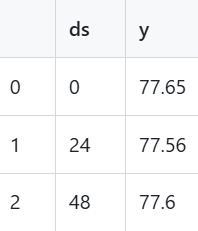
\includegraphics[scale=0.6]{sec/No.4data.png} % 替换为你的图片文件名
   %\includegraphics[width=0.8\linewidth]{egfigure.eps}

   \caption{No4.Data.
  ds represents the time interval in hours and y represents the current.}
   \label{fig:onecol}
\end{figure}

\begin{figure}[H]
  \centering
     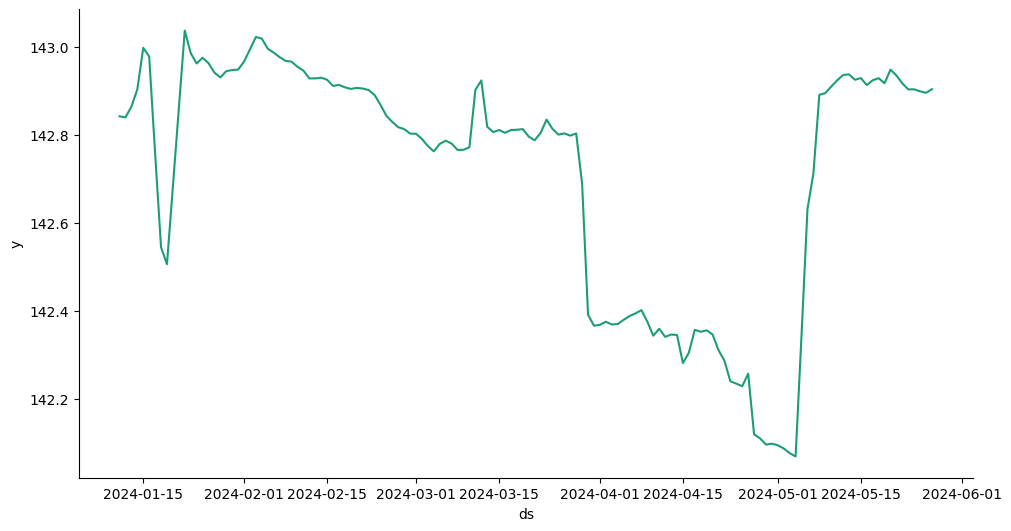
\includegraphics[width=\linewidth]{sec/No.3data.png} % 替换为你的图片文件名
   %\includegraphics[width=0.8\linewidth]{egfigure.eps}

   \caption{Visualization of Data for Component No. 3.
  ds represents the date and y represents the current.}
   \label{fig:onecol}
\end{figure}

\section{Proposed Innovations}
\label{sec:innovation}
%本实验的创新点分为数据集创新和算法创新。其中数据集创新方面由于本实验所用的数据集是组内成员采集的原创数据集因此数据集创新已经实现,而算法创新方面,拟通过修改调试实现Autoformer: %Decomposition Transformers with Auto-Correlation for Long-Term Series Forecasting及TIMESNET: TEMPORAL 2D-VARIATION MODELING FOR GENERAL TIME SERIES ANALYSIS论文中
%的方法,查看这两种方法在原创数据集上的效果,并与LSTM,RNN,TCN等传统方法对比,探索一种效果更好的方法。
The innovations in this experiment can be divided into two aspects: dataset innovation and algorithm innovation.

For dataset innovation, since the dataset used in this experiment is an original dataset collected by team members, the innovation in this aspect has already been achieved.

For algorithm innovation, the experiment aims to modify and debug methods proposed in the papers "Autoformer\cite{NEURIPS2021_bcc0d400}: Decomposition Transformers with Auto-Correlation for Long-Term Series Forecasting" and "TimesNet\cite{DBLP:journals/corr/abs-2210-02186}: Temporal 2D-Variation Modeling for General Time Series Analysis", to evaluate their performance on the original dataset. The results will then be compared with traditional methods such as LSTM, RNN, and TCN, in order to explore an approache with superior performance.

%\section{Final copy}

You must include your signed IEEE copyright release form when you submit your finished paper.
We MUST have this form before your paper can be published in the proceedings.

Please direct any questions to the production editor in charge of these proceedings at the IEEE Computer Society Press:
\url{https://www.computer.org/about/contact}.
{
    \small
    \bibliographystyle{ieeenat_fullname}
    \bibliography{main}
}

% WARNING: do not forget to delete the supplementary pages from your submission 
% \clearpage
\setcounter{page}{1}
\maketitlesupplementary


\section{Rationale}
\label{sec:rationale}
% 
Having the supplementary compiled together with the main paper means that:
% 
\begin{itemize}
\item The supplementary can back-reference sections of the main paper, for example, we can refer to \cref{sec:intro};
\item The main paper can forward reference sub-sections within the supplementary explicitly (e.g. referring to a particular experiment); 
\item When submitted to arXiv, the supplementary will already included at the end of the paper.
\end{itemize}
% 
To split the supplementary pages from the main paper, you can use \href{https://support.apple.com/en-ca/guide/preview/prvw11793/mac#:~:text=Delete%20a%20page%20from%20a,or%20choose%20Edit%20%3E%20Delete).}{Preview (on macOS)}, \href{https://www.adobe.com/acrobat/how-to/delete-pages-from-pdf.html#:~:text=Choose%20%E2%80%9CTools%E2%80%9D%20%3E%20%E2%80%9COrganize,or%20pages%20from%20the%20file.}{Adobe Acrobat} (on all OSs), as well as \href{https://superuser.com/questions/517986/is-it-possible-to-delete-some-pages-of-a-pdf-document}{command line tools}.
\end{document}
